% !TEX root = raport.tex
\documentclass{article}
\usepackage{polski}

\usepackage{amssymb}
\usepackage{amsmath}
\usepackage{mathtools}
\usepackage{graphicx}
\usepackage{booktabs}
\usepackage{caption}
\usepackage{pgfplotstable}
\usepackage{pgffor} 
\usepackage{float}
\usepackage{etoolbox}
\usepackage{pgf}

\pgfplotsset{compat=1.18}
\usepackage{hyperref}
% \usepackage{emoji}
\usepackage[includehead, left = 2cm, right = 2cm, top = 0.5cm, bottom = 2.45cm, includefoot, headheight = 10mm, footskip = 5mm]{geometry}

\setlength{\parindent}{0pt}
\usepackage{fancyhdr}

\pagestyle{fancy}
\fancyhf{} % clear default
\lhead{\textbf{Piotr Sitek}} % change to your name
\rhead{\textbf{fourth\_miniproject}}
\renewcommand{\headrulewidth}{1pt} % horizontal line thickness

\begin{document}

  \section*{Klasteryzacja}

  Zaimplementowałem klasteryzację hierarchiczną, metodą $k$-średnich oraz spektralną.

  \vspace{5pt}

  Na początku nie stosowałem algorytmu Lance'a Williamsa przez co klastrowanie hierarchiczne trwało bardzo długo.
  Po zastosowaniu go przyśpieszyło drastycznie (z $1min\ 26s$ do około $1.2s$ na zbiorze \texttt{rp.data}).

  \vspace{5pt}

  Klasyfikatory oparte na klastrowaniu sprawdzały się dobrze na pliku \texttt{rp.data}. 
  % Oto uzyskane 
  Nie stosowałem funkcji jądrowych.
  Wyniki dla liczby klastrów równej liczbie cech są przedstawione \hyperref[tab:clustering-accuracy]{tutaj}.

  \vspace{5pt}

  % \begin{minipage}{\textwidth}
  %   
\includegraphics[width=0.49\textwidth]{"./Images/Hierarchical.png"}
  %   
\includegraphics[width=0.49\textwidth]{"./Images/KMeans and Spectral.png"}
  % \end{minipage}

  \vspace{5pt}

  Następnie spróbowałem dla każdego datasetu 
  (poza \texttt{2D\_5} bo jest ich dużo więc obliczenia byłyby długie)
  dobrać optymalną liczbę klastrów.

  \vspace{5pt}
  
  Narysowałem wykresy błędu zdefiniowanego na slajdzie z KMeans w zależności od liczby 
  klastrów i użyłem na tym reguły łokcia.

  \vspace{5pt}

  Oto uzyskane wykresy:

  \vspace{5pt}
  \begin{center}
    \newcommand{\imwidth}{0.28\linewidth}

    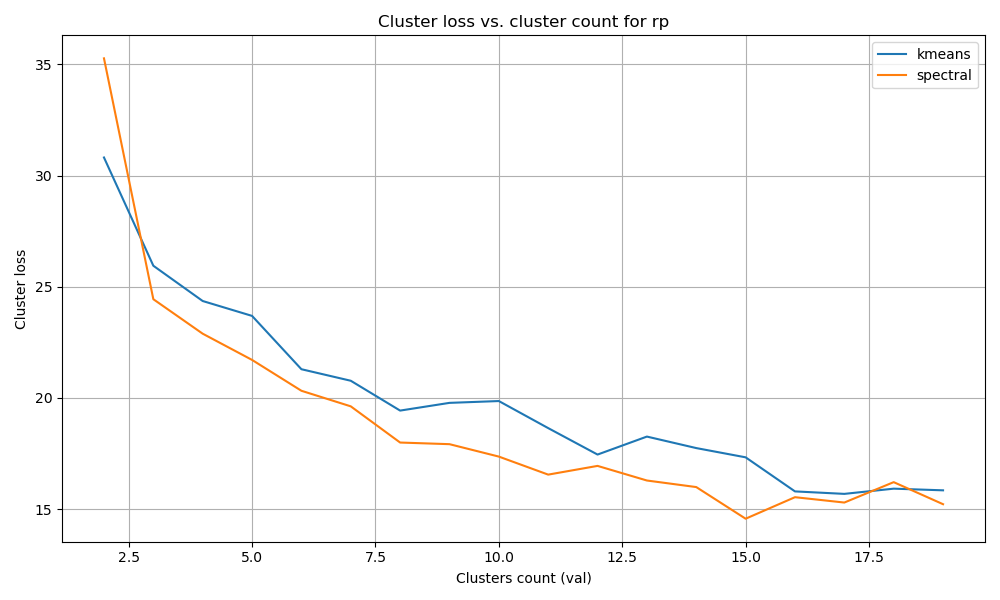
\includegraphics[width=\imwidth]{Images/Elbow/inertion_of_rp.png}
    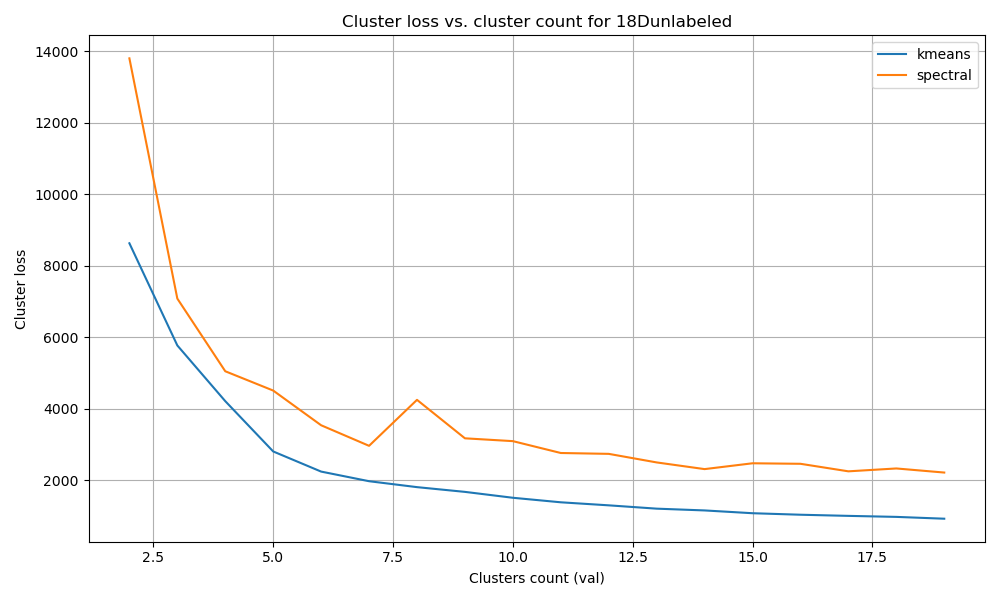
\includegraphics[width=\imwidth{}]{Images/Elbow/inertion_of_18Dunlabeled.png}
    \newcounter{temp} % define a new counter
    \setcounter{temp}{0} % set initial value
    \foreach \i in {1,...,8} {
    % \begin{minipage}{\textwidth}
      \ifnumcomp{\i}{=}{5}{
        }{
          \pgfmathparse{mod(\value{temp},3)==1}
          \ifnum\pgfmathresult=1
            \vspace{5pt}
            \\
          \fi
          \includegraphics[width=\imwidth]{Images/Elbow/inertion_of_2D_\i.png}
          \stepcounter{temp}
        }
    % \end{minipage}
      }
  \end{center}

  Nie sprawdzałem błędów dla klastrowania hierarchicznego bo było istotnie wolniejsze od alternatyw. 

  \vspace{5pt}

  Na podstawie tych wykresów wyznaczyłem liczby klastrów dla każdego z plików \texttt{dane\_2D\_i.txt}.

  \vspace{5pt}

  Po uruchomieniu modeli na danych dwuwymiarowych z liczbą klastrów równą $2*\textit{liczba różnych etykiet}$ 
  oraz z~dobraną przeze mnie liczbą klastrów otrzymałem podobne lub trochę lepsze wyniki na liczbach dobranych 
  przez siebie. Wyjątkiem jest dataset \texttt{data2D\_6} gdzie dobrałem mniej klastrów niż jest cech ($10$ zamiast $15$)
  i~precyzja spadła z~$99\%$ do $66\%$.

\begin{table}[ht!]
  \centering
  \label{tab:clustering-accuracy}
  \captionof{table}{Classification Accuracy per Model and Dataset}
  \pgfplotstableread[col sep=comma]{\detokenize{Data/best_results.csv}}\loadedtable

  \pgfplotstabletypeset[
    columns/dataset/.style={string type},
    every head row/.style={before row=\toprule, after row=\midrule},
    every last row/.style={after row=\bottomrule},
    fixed zerofill,
    precision=4,
  ]{\loadedtable}


  % \pagebreak
  \captionof{table}{Training times per Model and Dataset in seconds}

  \pgfplotstableread[col sep=comma]{\detokenize{Data/times.csv}}\loadedtable

  \pgfplotstabletypeset[
    columns/dataset/.style={string type},
    every head row/.style={before row=\toprule, after row=\midrule},
    every last row/.style={after row=\bottomrule},
    fixed zerofill,
    precision=4,
  ]{\loadedtable}

\end{table}

\vspace{5pt}

Z wyników można wywnioskować, że klastrowanie za pomocą łączenia pojedynczego (min-linking) generalnie sprawdza się gorzej
od innych rodzajów klastrowania ale są datasety (\texttt{\detokenize{dane2D_4.txt}}) których specyfika sprawia, że działa ono zdecydowanie
lepiej od innych.

\vspace{5pt}

Można też zauważyć, że klastrowanie spektralne daje gorsze wyniki od hierarchicznego oraz kmeans ale jest szybsze na małych danych.

\vspace{5pt}

Poniżej zamieszczam $2$ wizualizacje przedstawiające działanie zaimplementowanych 
algorytmów klasteryzacji na dwuwymiarowych danych. Pierwsza przedstawia klastry rozróżnione na drodze 
klastrowania a druga przypisanie etykiet do punktów.


\vspace{5pt}

\foreach \i in {1,...,8} {
  % \begin{minipage}{\textwidth}
      \subsubsection*{Dataset 2D\_\i}

      \renewcommand{\figurename}{All clusters}
      \begin{figure}[H]
        \centering
        \includegraphics[width=0.8\linewidth]{{Images/2D_visualizations/2D_\i.png}}
        \caption{{Dataset \texttt{2D\_\i}}}
      \end{figure}

      \renewcommand{\figurename}{Classification results}
      \begin{figure}[H]
        \centering
        \includegraphics[width=0.8\linewidth]{{Images/2D_visualizations/correct_colors_2D_\i.png}}
        \caption{{Dataset \texttt{2D\_\i}}}
      \end{figure}
  % \end{minipage}
}

\end{document}
